\documentclass[fleqn]{article}
\usepackage[margin=1in]{geometry}
\usepackage[nodisplayskipstretch]{setspace}
\usepackage{amsmath, nccmath, bm}
\usepackage{amssymb}
\usepackage{enumitem}
\usepackage{graphicx}
\usepackage{float}

\newcommand{\zerodisplayskip}{
	\setlength{\abovedisplayskip}{0pt}%
	\setlength{\belowdisplayskip}{0pt}%
	\setlength{\abovedisplayshortskip}{0pt}%
	\setlength{\belowdisplayshortskip}{0pt}%
	\setlength{\mathindent}{0pt}}
	
\title{Homework 1}
\author{Owen Sowatzke}
\date{February 9, 2025}

\begin{document}

	\offinterlineskip
	\setlength{\lineskip}{12pt}
	\zerodisplayskip
	\maketitle
	
	\begin{enumerate}
		\item Given below is an illustrative layout of an inverter. Write down the material layer used according to color and arrange them in the order of fabrication.
		
		\begin{figure}[H]				
			\centerline{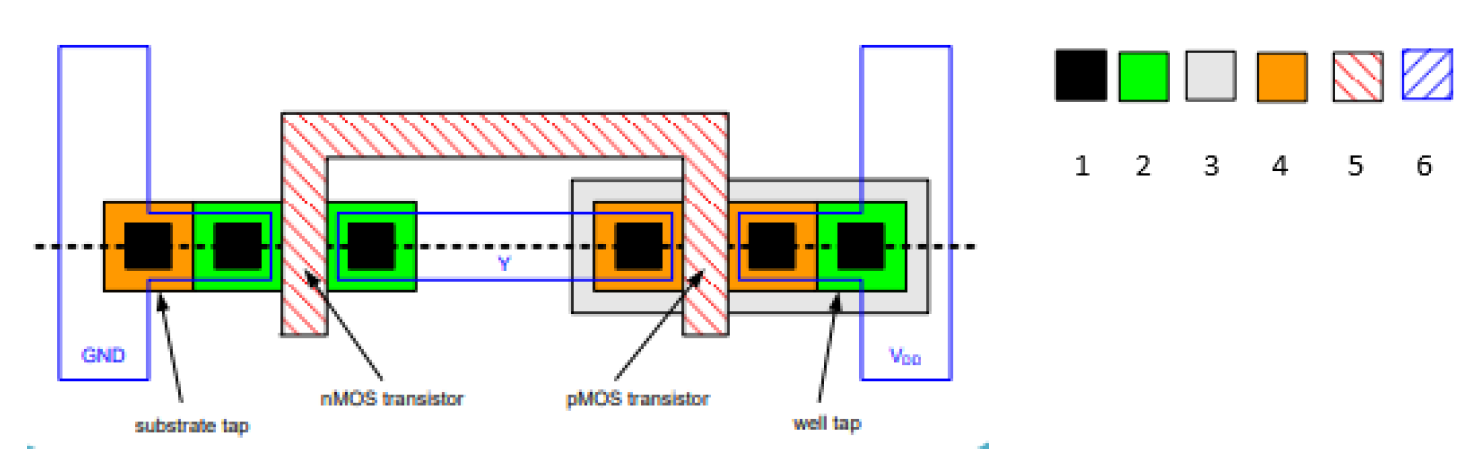
\includegraphics[width=0.8\textwidth]{inverter_layout.png}}
			\label{fig::inverter_layout}
		\end{figure}
		
		The materials in the layout are defined as follows:
		
		\begin{itemize}
			\item Material 1 (solid black) is contact material. It is made of metal (usually aluminum).
			\item Material 2 (solid green) is n+ diffusion (heavily doped n-type semiconductor [usually Si])
			\item Material 3 (solid gray) is the n-well (lightly doped n-type semiconductor [usually Si])
			\item Material 4 (solid orange) is the p+ diffusion (heavily doped p-type semiconductor [usually Si])
			\item Material 5 (striped red) is the polysilicon.
			\item Material 6 (striped blue) is the metal1 (usually aluminum)
		\end{itemize}
		
		The material layers are fabricated from the bottom up in the following order:
		
		\begin{enumerate}
			\item[1.] Material 3 (the n-well)
			\item[2.] Material 5 (polysilicon)
			\item[3.] Material 2 (n+ diffusion)
			\item[4.] Material 3 (p+ diffusion)
			\item[5.] Material 1 (contact)
			\item[6.] Material 6 (metal1)
		\end{enumerate}
		
		\item Illustrate the CMOS Layout and Stick diagram for the following Boolean expressions.
		
		\begin{enumerate}
			\item $Y = (A+B)\cdot(C+D)$
			
			In CMOS circuit design, we implement circuits that are the complement of boolean expressions. Because the provided expression is not in complement form, we must design a circuit to get $\bar{Y}$ and append an inverter to get $Y$.
			
			We start by designing the pull-down circuit to get $\bar{Y}$. We replace each "or" with a parallel set of nmos gates and each "and" with a series of nmos gates. The pull-down circuit is shown in the bottom half of Figure \ref{fig::cmos_layout_problem_2a}. We can then use the rule of conduction complements to design the pull-up circuit. To do so, we replace each parallel set of nmos gates with a series of pmos gates and each series of nmos gates with a parallel set of nmos gates. The resulting pull-up circuit is shown in the top half of Figure \ref{fig::cmos_layout_problem_2a}. The output $\bar{Y}$ is then fed into an inverter to get $Y$.
			
			\begin{figure}[H]
				\centerline{\fbox{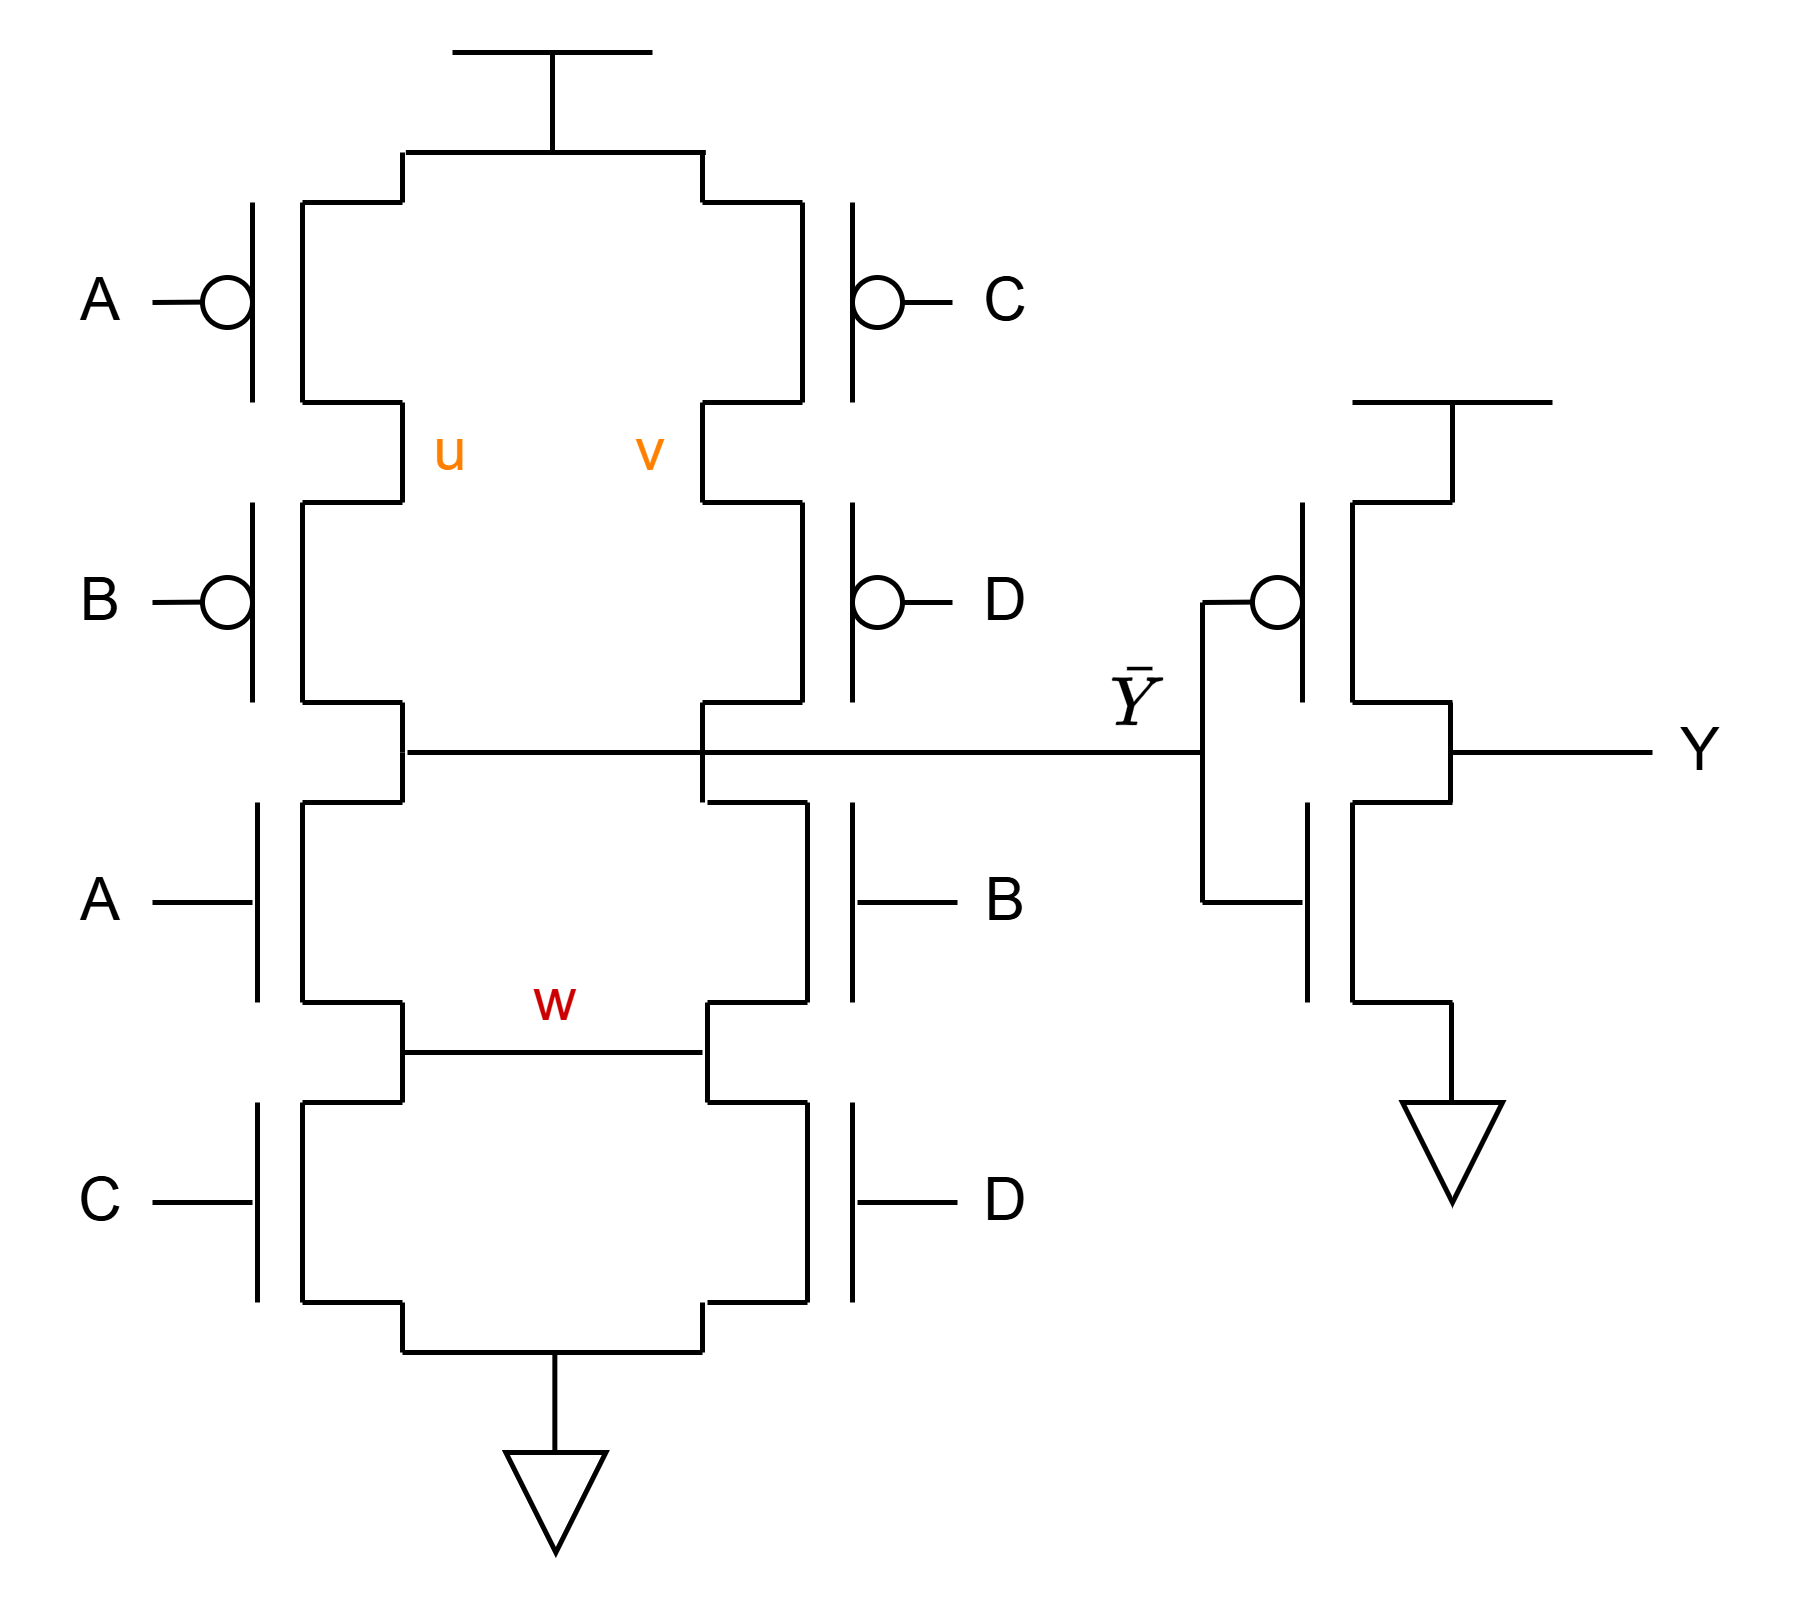
\includegraphics[width=0.5\textwidth]{cmos_layout_problem_2a.png}}}
				\caption{CMOS Layout for Problem 2a}
				\label{fig::cmos_layout_problem_2a}
			\end{figure}
			
			To determine the order of the stick diagram inputs, we must find a Euler Path through the circuit. The Euler Path for this circuit has been traced out in the logic diagram shown in Figure \ref{fig::logic_diagram_problem_2a}.
			
			\begin{figure}[H]
				\centerline{\fbox{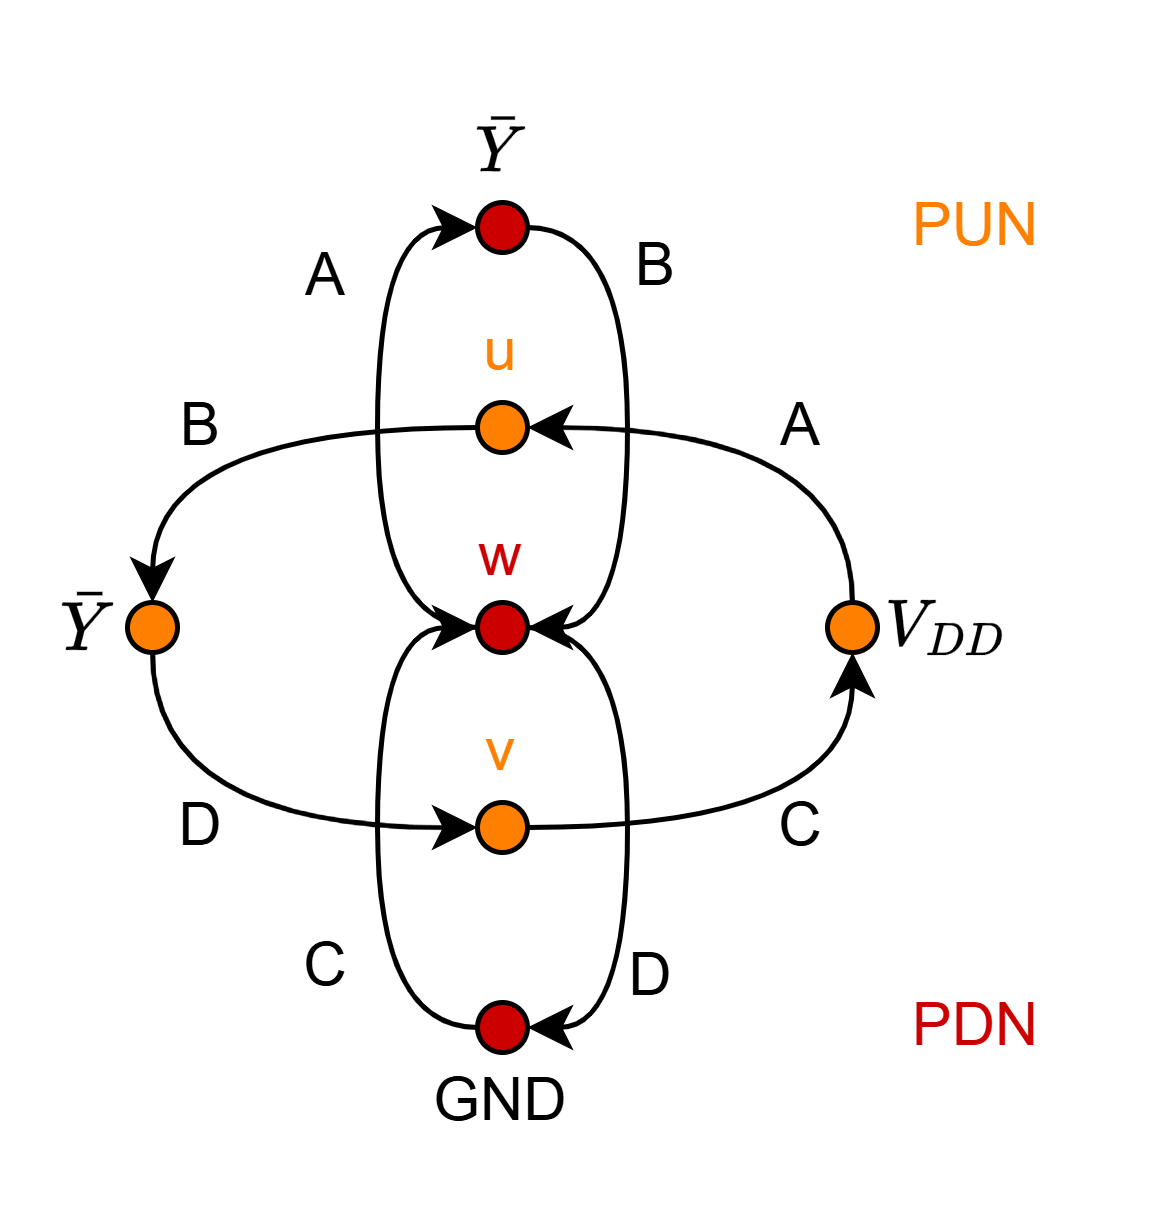
\includegraphics[width=0.4\textwidth]{logic_diagram_problem_2a.png}}}
				\caption{Logic Diagram for Problem 2a Illustrating Euler Path}
				\label{fig::logic_diagram_problem_2a}
			\end{figure}
			
			The Euler path can be found by independently tracing through all the nodes of the pull-down and pull-up networks once and only once. The path we find must also be consistent between the pull-up and pull-down networks. For this example, we determine the following input ordering: A, B, D, C. This ordering we find using the Euler path helps us generate a layout without diffusion breaks. Using the requested input ordering, we come up with the stick diagram shown in Figure \ref{fig::stick_diagram_problem_2a}. Note that we have also added an inverter to get $Y$ instead of $\bar{Y}$
			
			\begin{figure}[H]
				\centerline{\fbox{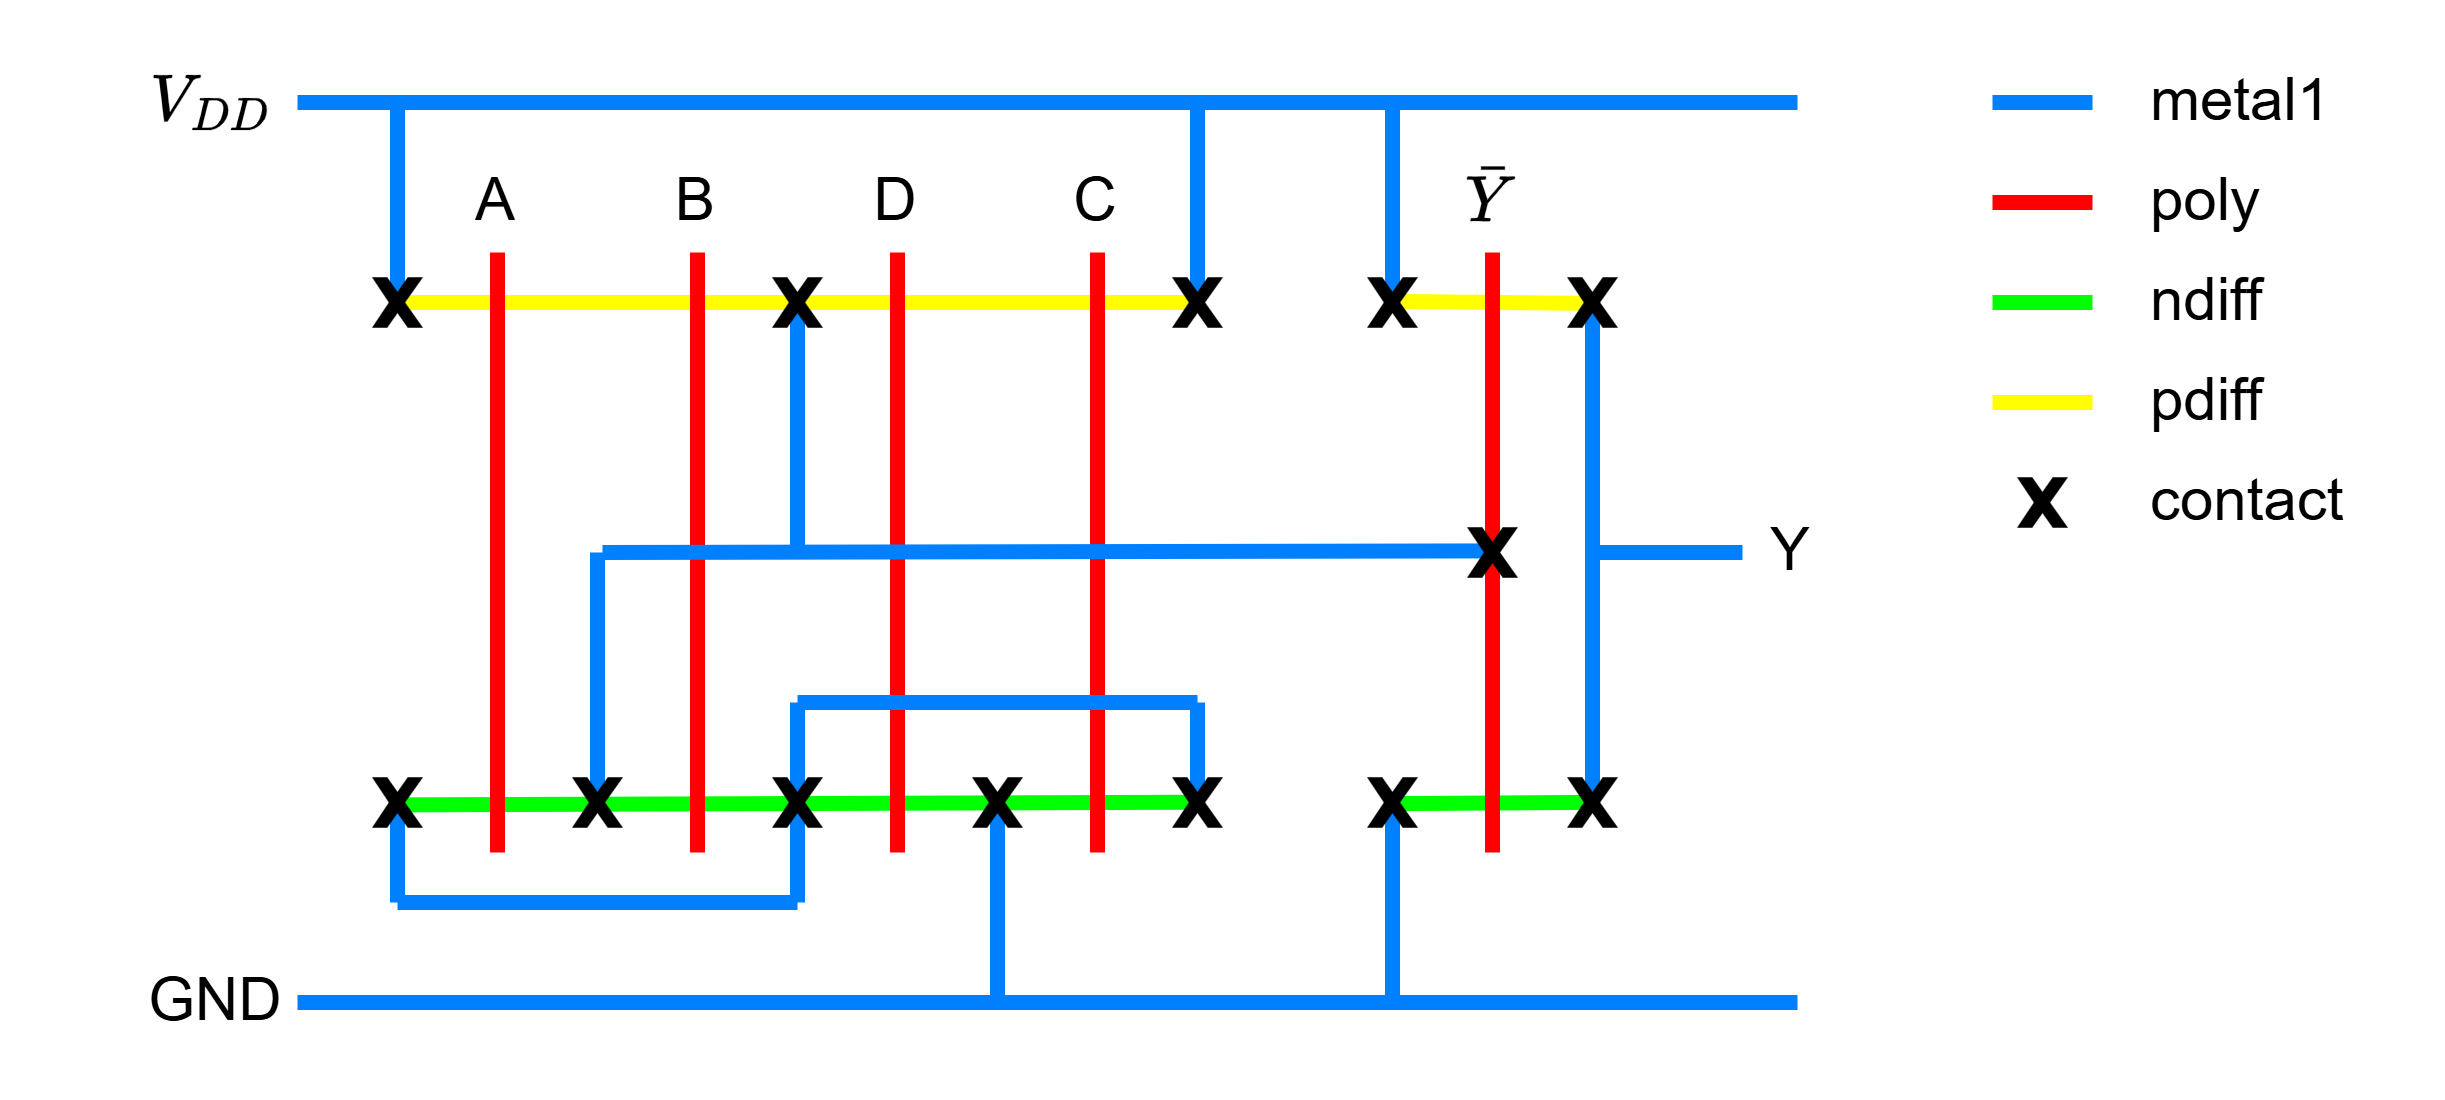
\includegraphics[width=0.6\textwidth]{stick_diagram_problem_2a.png}}}
				\caption{Stick Diagram for Problem 2a}
				\label{fig::stick_diagram_problem_2a}
			\end{figure}
			
			\item $Y = \overline{A \cdot B + C \cdot D}$
		\end{enumerate}
	\end{enumerate}
\end{document}